\section{Effectiveness of \plink}
We continue to evaluate \plink in public cloud environments. 

Our evaluation goals are as follows: (1) Measure \plink{}'s impact on end-to-end training.  (2) Demonstrate the efficiency of \ha. (3) Quantify the benefit of hierarchical aggregation and topology-awareness. (4) Evaluate the accuracy of \marcopolo{}'s inference of physical affinity. (5) Assess how well \autoplink reacts to network changes. 

\subsection{Environment Setup}
\label{sec:commBackend}
We perform our experiments on both \azure and \ectwo, in the same region or availability zone. Each VM runs Linux kernel 4.18 with SoftiWarp support~\cite{zrliosof32:online}, Cuda 9.2, CuDNN 7, and network enhancements~\cite{Createan37:online, Enablean80:online} if possible. All VMs are provided with at least 10~Gbps network throughput, using DCTCP~\cite{data-center-tcp-dctcp} as SoftRoCE and SoftiWarp do not yield better performance. \ha uses a chunk size tuned to its best performance, usually 16 to 64KB. All experiments use 64 nodes unless otherwise specified. Some experiments involve comparing results generated with uncertainty. In those cases, we report speedup in terms of mean and percentile metrics together with performance distribution of 50 runs. Each sample represents mean performance of 20 iterations using a potentially different cluster assignment generated by the underlying mechanism. %, and each sample collected is the mean performance of 20 iterations. %We also interleave runs of different approaches to further reduce the interference from the environment, as suggested in~\cite{perfVariance}.

%To find the fastest transport layer for \ha, we use a benchmark that measures the median latency of 50 reduction runs of 512MB of data (sufficiently large for throughput measurement), on C5 and Standard D VMs on EC2 and Azure. We found our TCP implementation to be 1.07x and 5.94x faster than SoftiWarp and SoftRoCE implementations. We also found no significant performance differences among various TCP variants. In the following performance experiments, we use DCTCP~\cite{data-center-tcp-dctcp} as it keeps queueing delays low within a datacenter. To ensure our baselines get the best performance, we enforce all VMs to be in the same availability zone on EC2 and the same datacenter on Azure. \textsection\ref{sec:related} discusses the potential of \plink to accelerate cross-datacenter, cross-region training. In accuracy measurements, we allow VMs to span more hierarchy for a wider coverage.

%Some experiments report aggregation-only performance, and the setup will be specified individually. Some report end to end training performance of training popular neural network models in terms of throughput speedup. We omit accuracy result, as \plink optimizations do not change this. We found no big difference in throughput when training with Pytorch/Caffe2 or MxNet. Thus we report only Pytorch/Caffe2 performance. 
%We fit 8 samples/GPU. We did not use large batch optimizations in order to stress the communication part of the training pipeline without oversaturating the GPUs. See \ref{sec:related} for a discussion.

\begin{figure}[t!]
	\centering
	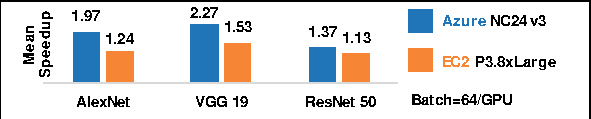
\includegraphics[width=.7\linewidth, trim=2 1 1 3,clip]{Figures/end2end.pdf}
	\caption{\plink{}'s collective optimizations achieve up to 2.27x speedup on  public clouds training popular neural network models, compared to original Pytorch/Caffe2.}
	\label{fig:end2end}
\end{figure}


\subsection{End to end training performance}
We start our evaluation with the impact of \plink{}'s collective optimizations on the end-to-end training performance of popular neural networks. Then we breakdown the effect of each optimization in the following sections. We compare \plink{} to original Pytorch/Caffe2 performance by replacing Gloo. We represent training speedup as mean speedup in throughput of 50 iterations to save experimental cost. This directly translates to a reduction in end-to-end training time as \plink{}'s optimization does not change convergence because it keeps the computation intact. %We use a batch size of 64/GPU on 64 P3.8xLarge nodes on \ectwo and Standard NC24v3 nodes on \azure, each with a V100 GPU. We simply generate 8 clusters with balance elasticity set to 2.

Figure~\ref{fig:end2end} shows the speedup of \plink, which ranges from 1.37-2.27x on \azure, and 1.13x-1.53x on \ectwo\footnote{While we report only data-parallel results for its dominance in distributed training, \plink optimizations are paradigm-agnostic, as all the scheduling of transfers is done by the framework.} when training popular vision models. We expect larger speedups for neural networks with higher communication to computation ratios (such as AlexNet and VGG) on VMs with faster networks, as we observe near line-rate network utilization when training them with \plink. For models with smaller communication to computation ratios (such as ResNet-50), \plink{}'s speedup comes from its reduced reduction latency.

\subsection{Efficiency of \ha}
\label{sec:baseline}
This section evaluates the performance of \ha itself, disabling \marcopolo{} and \autoplink{}. %. In particular we examine the performance gains achieved by \ha{} from efficient execution of aggregation schedules. % while \ref{sec:2lhaRandom} reveals the additional speedup from a \strongrandom-powered hierarchical scheme.
%\noindent\textbf{Comparison to other systems.}
For clarity, we first set up our baseline with communication libraries used in major training frameworks, including MxNet PS-Lite, Nvidia NCCL 2.4, and Facebook Gloo, covering ring (Gloo, NCCL), tree (NCCL), halving-doubling (Gloo) and parameter server (PS-Lite). %(\textsection\ref{sec:differentReductionAlgorithms}).
We use each library's benchmark program to measure its performance. On both \azure and \ectwo, we use instances with V100 GPUs and test end-to-end reduction performance
%~\cite{dmlcpsli50:online}
involving copying from/to a GPU. % The rest of experiment setup is same as in \textsection\ref{sec:commBackend}.

\begin{figure}[t!]
	\centering
	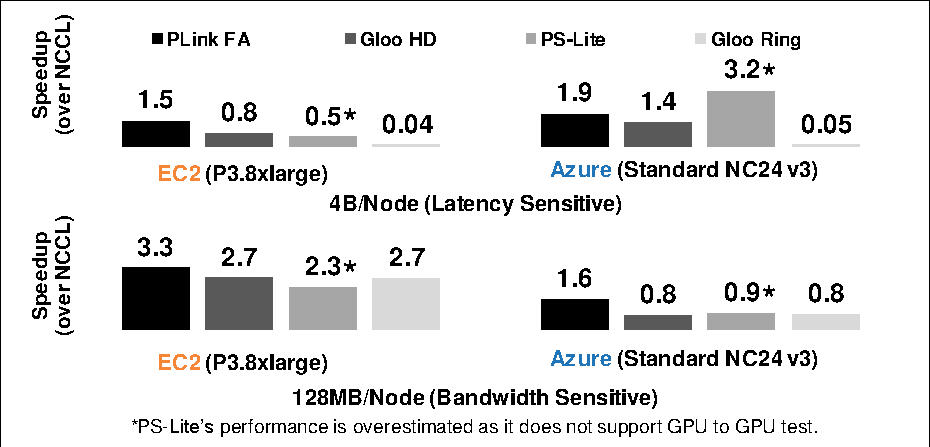
\includegraphics[width=.7\linewidth, trim=2 3 3 3,clip]{Figures/baseline.pdf}
	\caption{GPU to GPU aggregation speedup of various systems on \azure and \ectwo in terms of mean latency for large and small buffers, normalized to NCCL's performance. }
	\label{fig:baseline}
\end{figure}

\begin{figure}[t!]
	\centering
	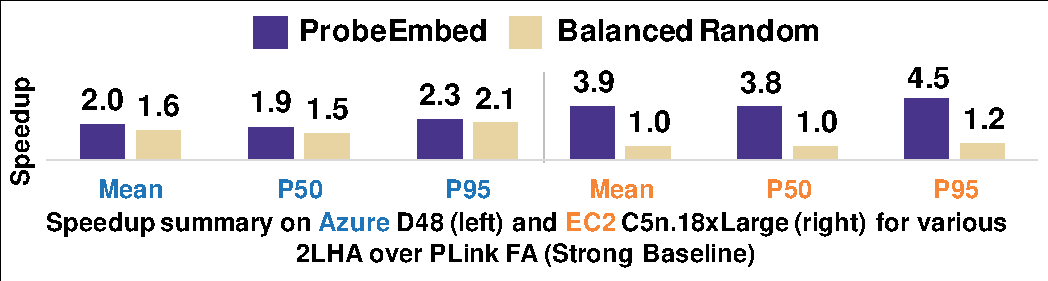
\includegraphics[width=.7\linewidth, trim=2 3 3 3,clip]{Figures/perfSummary.pdf}
	\caption{Mean, P50, and P95 additional speedup of \mlha using different approaches over FA (\strongbaseline). Run on 64 \azure D64 series and \ectwo C5n.18xLarge instances, with a constant VM topology throughout this experiment.}% See detailed analysis for each series in corresponding sections. ResNet-50 buffer sizes and distributions is used.}
	\label{fig:perfSummary}
\end{figure}

Figure \ref{fig:baseline} shows the speedup in terms of mean (20 iterations) GPU to GPU reduction latency normalized to NCCL's result of aggregating a large (128MB) and a small (4B) buffer. To provide a fair comparison, we limit \ha to use a single connection per peer (in a typical scenario, multiple connections are used). Overall, \ha{}'s flat aggregation (FA) leads the pack and is thus used as a \strongbaseline.

%\begin{table}
%        \centering
%        \footnotesize
%	\begin{tabular}{|c|c|c|c|c|c|c|}
%		\hline
%		Time (ms)   & 2 nodes & 4 & 8 & 16 & 32 & 64 \\
%		\hline
%		EC2  & 535   & 680   & 923  &  951 & 1270 & 1247  \\
%		\hline
%		Azure & 937 & 961 & 967 & 989 & 934 & 1031 \\
%		\hline
%	\end{tabular}
%	\caption{Reduction latency (512MB/node) vs number of nodes.}
%	\label{table:scalability}
%\end{table}

%\noindent\textbf{Scalability.}
%\label{sec:scalability} We also evaluated \ha{}'s scalability by varying the number of participating nodes on Azure, with a buffer size of 512MB. \ha achieves a 91\% scaling ratio from 2 to 64 nodes. This is because \ha{}'s chunking (\textsection\ref{sec:generatingAggregationPlan}) capability keeps per-node workload constant.

%The bumps of latency on EC2 as we add nodes is likely due to nodes are more spread as they are added in, as the latency of each iteration is determined by the bottleneck link in the full connection mesh. 
%so ideally, the reduction latency should not increase if each node can achieve full bandwidth goodput when communicating with rest of the nodes. Second, we notice the bumps of latency from 4 to 8 and 16 to 36 nodes on EC2, likely due to nodes are more spread as more are added in.

%\begin{table}
%        \centering
%        \footnotesize
%	\begin{tabular}{|c|c|c|c|}
%		\hline
%		Speedup   & \strongrandom  & Groundtruth & \marcopolo{}  \\
%		\hline
%		EC2  & 2.47   &  N/A   & 3.09   \\
%		\hline
%		Azure & 1.20 & 1.16 & 1.32\\
%		\hline
%	\end{tabular}
%	\caption{Aggregated relative speedup over FA (\strongbaseline) achieved on 64 Azure F16 series and EC2 C5n.18xlarge instances, with a constant VM topology throughout this experiment. See detailed analysis for each column in corresponding sections.}
%	\label{table:perfSummary}
%\end{table}

\subsection{Effectiveness of Hierarchical Aggregation}
\label{sec:2lhaRandom} 
We continue with a detailed comparison between \plink FA and \mlha, reducing a real-world model (ResNet-50, varying buffer sizes totalling~$\approx$100MB). We use 4 connections per peer to fully utilize VM bandwidth. We separately tuned chunk sizes to ensure baseline perform well in both clouds. We present the speedup summary in Figure~\ref{fig:perfSummary}; then, each subsection details the benefits associated with the individual technique. Performance distribution is found in Figure~\ref{fig:probeembedvsrandomvsflat}.  %Overall, \plink{} is able to achieve up to 4x mean and 4.5x P95 (95th percentile) speedup on \ectwo, and 2x mean and 2.3x P95 speedup on \azure compared to FA. 

%\subsubsection{\strongrandom-guided \mlha versus FA}
%\mlha can provide a performance benefit over FA without takig network locality into account by using \textit{\strongrandom}~(\textsection\ref{sec:marcopolo}) to generate schedules.  Figure \ref{fig:probeembedvsrandomvsflat} shows that, empirically, \strongrandom HA can achieve a mean speedup of 1.6x on \azure over FA, and is on par with FA's mean performance with shorter tail on \ectwo, whereas FA performance is highly volatile due to its sensitivity to network conditions as nodes communicate in an all-to-all pattern. %HA performance varies due to variability in the specific clusters generated for each run. Nonetheless, HA achieves both a lower expected reduction latency and a lower tail latency due to more localized communication.

%To improve our coverage, we ran the same experiments in additional configurations on Azure and EC2 (e.g., using the F, NC and E instances on Azure as well as G3 and P3 instances on EC2) and observed similar benefits. %Across all our experiments, on Azure, random \mlha performance beats FA by up to 1.7x; on EC2, the speedup is up to 3.9x. 
% Only in few cases do we fail to see a meaningful speedup of \mlha over FA.
%The speedup of random \mlha over FA comes from the traffic localization property of HA: only one copy of the buffer is transferred intercluster.
%While it is impractical to sample random performance across all physical configurations and clustering, we summarize our empirical finding on 64 Azure Standard F, Standard DS and Standard NC series VMs, as well as G3, C5 and P3 instances on EC2: 


\begin{figure}
	\centering
	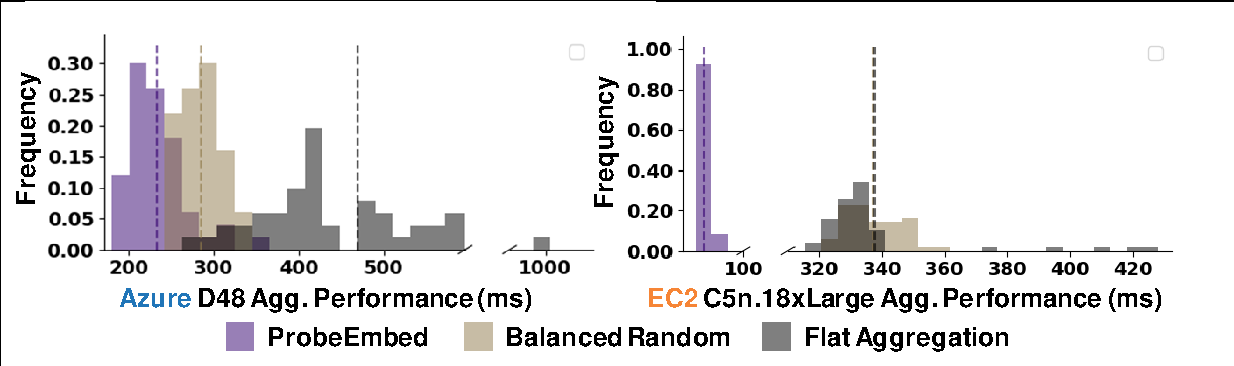
\includegraphics[width=.7\linewidth, trim=2 5 20 20,clip]{Figures/probeembedvsrandomvsflat.pdf}
	\caption{Empirical reduction latency distribution of \marcopolo-, \strongrandom- guided \mlha and FA on \azure and \ectwo.}
	\label{fig:probeembedvsrandomvsflat}
\end{figure}

%\subsubsection{\marcopolo{}'s Impact on \mlha Performance} This section highlights the benefit and necessity of \marcopolo{}, by comparing \marcopolo{}-guided \mlha with schedules crafted using ground-truth and \strongrandom.

\noindent\textbf{Comparing with ground-truth-guided \mlha.}
% \footnote{We did not obtain ground-truth information from EC2. However, we did experiments on EC2 that focused on inferring availability zone difference. Our high performance results in these experiments are unremarkable because cross availability zone communication has drastically higher latency.}, and focus our evaluation on Azure in this section.
Cloud providers can expose topology information to assist in locality-aware scheduling and communication. We obtain ground-truth topology information from \azure. We look at the effectiveness of using physical topology on \azure to form a reduction schedule for \mlha, grouping VM nodes based on their physical locality. % they are located in. %\arvind{are we saying that we don't group VMs inside a cluster for instance?  is the point that the cloud provider is providing only rack-level topo info?}


%We cluster nodes based on their physical residence (racks in this experiment). We used 64 Azure F instances for this experiment. In each run, the groundtruth-based clustering is fixed, while \marcopolo{} may generate different clusters. Thus we present speedup in terms of a measured performance distribution. The rest of the setup is kept the same as \ref{sec:2lhaRandom}.

%\begin{figure}
%	\centering
%	\includegraphics[width=\linewidth, trim=10 5 10 20,clip]{Figures/vsgroundtruth.pdf}
%	\caption{Empirical reduction performance distribution with \marcopolo{}-based clustering and groundtruth based clustering on two different spawns of 64 Azure F instances. \marcopolo{} leads groundtruth performance by 1.9x and 2x, and has lower performance variance.}
%	\label{fig:vsgroundtruth}
%\end{figure}

%We respawn the VMs multiple times to obtain different topologies in order to understand how they affect \mlha performance. For the runs shown in Figure~\ref{fig:perfSummary}, \marcopolo-guided \mlha beats ground-truth-guided \mlha by 7.1x for Azure (which is the setting where we were able to obtain ground-truth data). % and these 64 VMs are spread across 22 racks, with the largest rack containing 8 VM nodes while the smallest containing only 1. In two other occasions, these 64 VMs landed in 17 racks and 40 racks respectively, and \marcopolo{} achieves 1.9x and 2.0x speedup over ground-truth-guided approach.

Our experiment shows that \marcopolo-guided \mlha beats ground-truth-guided \mlha by 1.15x on average. The performance of ground-truth-guided \mlha relies on a ``luck'' factor related to the physical topology of the VM nodes: the more compactly the VMs are allocated, and the more balanced the allocation in each rack is, the better performance of ground-truth-guided \mlha should be. But VM spawn location is in total control of the scheduler, and sometimes it is impossible to guarantee a compact allocation due to current VM occupancy. It is difficult to splice/split undersized/oversized racks for a more balanced \mlha without probing for network properties, which \marcopolo{} does.


%\ref{fig:vsgroundtruth} illustrates this: a more compact allocation (64 VM nodes in 17 racks) does generate better performance and less variation than a more scattered allocation (64 VM nodes in 40 racks). But in both cases \marcopolo{}-guided \mlha beats groundtruth-guided \mlha by 1.9x and 2x respectively. Our further scrutiny shows the reason are (1) more compact allocation does not mean more balanced allocation, and without running network probes, it is difficult to splice or split undersized or oversized clusters to form a balanced \mlha plan, and (2) groundtruth-based approaches ignores completely the dynamic property of the network, which shifts how VM clusters are generated.

\noindent\textbf{Comparing with \strongrandom-guided \mlha.}
%marcopolo{}'s goals are to determine the number of clusters to generate, and returns clustered nodes. 
We observe an additional 1.3x and 3.9x expected performance gain of the clusters generated by \marcopolo{} over those of \strongrandom{} on \azure and \ectwo. \marcopolo{} leads to  better and more stable performance by generating cohesive, locality-preserving group assignments. On the other hand, \strongrandom can include VMs that are far away in the same group, creating a bottleneck in the system. %Our experience also indicates larger VM instances often have larger speedups with \marcopolo{}, perhaps because they are less likely to be packed into the same physical host, resulting in a low inherent locality. %, which is harder for \strongrandom to capture. %is likely to generate groups whose intra-group distance is similar to the diameter of the ring, by picking equally-spaced VM nodes on the circumference of the ring, which may result in lower variance but with less-than-ideal performance.

%One interesting observation is the three peaks in C5n's distribution. This may be due to the stochastic process of kmeans: for example, the lonely VM nodse on the upper-left can be partitioned into multiple clusters, resulting in different performance. Different initializations for the embedding process can also contribute to landing in different local minima in the optimization manifold.

%Across all experiments, we found \marcopolo{}-guided \mlha has a speedup range of 1.04x to 1.5x and 1.02 to 1.25x over random-guided \mlha on Azure and EC2, respectively. While \strongrandom can generate all possible clusters, \marcopolo{} effectively ''cherrypicks`` a smaller portion of the partitioning space that better preserves locality, leading to higher performance in expectation. Our experience also indicates larger VM instances often lead \marcopolo{} to have larger speedup gains, likely because they are less likely to be packed into the same physical host, causing VMs to spread across more physical hosts, resulting in less inherent locality, making it harder for \strongrandom to capture incidentally. % which \strongrandom is less likely to capture incidentally. %We also find larger instances usually lead to larger speedup, and this is likely due to the fact that smaller instances can be ''packed`` into a physical host, allowing more chance for \strongrandom to capture locality. In general, our observation indicates \marcopolo{}'s performance distribution has lower standard deviation compared to that of \strongrandom{}'s in general.


\begin{figure}
	\centering
	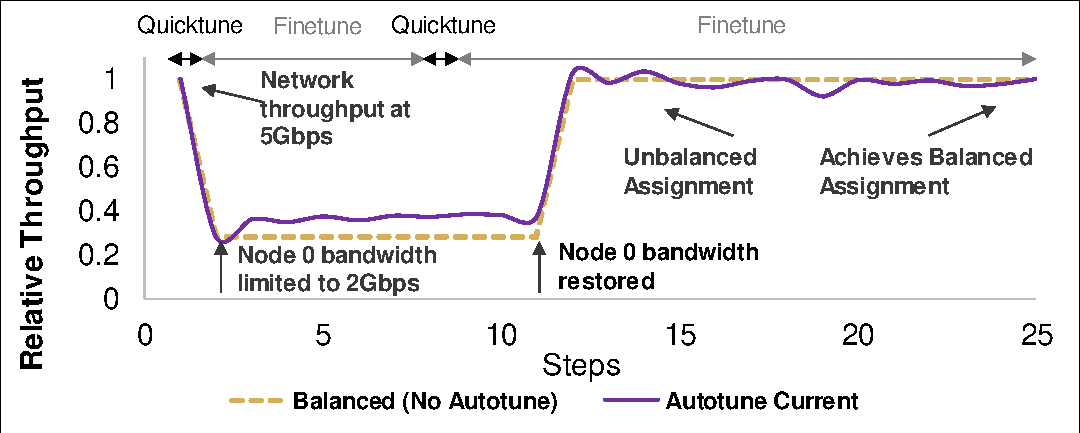
\includegraphics[width=.7\linewidth, trim=2 1 3 3,clip]{Figures/autotunebw.pdf}
	\caption{\autoplink adapts to bandwidth changes by assigning LMs based on current metrics of \ha. Dotted lines: averaged throughput. Solid lines: snapshot throughput.}
	\label{fig:autotunebw}
\end{figure}


%Surprisingly, we found \plink sustains a stable speedup of 1.5x on both Azure and EC2 with V100 GPUs, up to a batch size of 64 (at which point no more samples can be filled in). This suggests that with a fast modern GPU, memory becomes a bottleneck before computation, and thus \plink{}'s communication acceleration is valuable even with a large batch size. 



\subsection{Accuracy of \marcopolo{}}
\label{sec:accuracy}
Effective exploitation of locality requires capturing both static and dynamic aspects of the network (which is directly captured by the probes). %\marcopolo explicitly measures dynamic network properties and uses this information to infer static network topology. 
In this section, we evaluate \marcopolo{}'s ability to discover the network topology in terms of \textit{physical affinity}.
%from three angles: (1) the accuracy of different types of network probes; (2) the ability of \marcopolo{} to accurately infer VM physical affinity; and (3) the effectiveness of using embedding as a denoising technique.%(1) the accuracy of network probes used by \marcopolo{}; (2) the ability to accurately infer VM physical affinity and (3) the effectiveness of using embedding as a de-noising technique.

%\subsubsection{Physical Affinity Inference Accuracy (PAIA)}
\noindent\textbf{Physical Affinity Inference Accuracy (PAIA).}
We define \textit{affinity score} as an intuitive metric to quatify how well \marcopolo{} captures network topology: for any two VM nodes $(a,b)$ that have comparable distance to an observer $c$, let $T(a,c), T(b,c)$ be the ground-truth distance (in terms of hops) from $a$ to $c$ and $b$ to $c$, and let $M(a,c), M(b,c)$ be the \marcopolo{} measured distance. We define an affinity score $A(a,b,c)$ for triplet $(a,b,c)$ as:
%
\begin{align*}
\small
  A(a,b,c) = 
   \left\lbrace
  \begin{array}{l@{}l}
    1 \textbf{ if $M(a,c) < M(b,c)$ and $T(a,c) < T(b,c)$}\\
    \textbf{\quad or $M(a,c) > M(b,c)$ and $T(a,c) > T(b,c)$} \\
    0 \text{ otherwise}
  \end{array}
  \right.
\end{align*}

For a given $c$, $A(a,b,c)$ captures whether \marcopolo{}'s measurement agrees with the actual hop distance between $a$ and $b$. $A(a,b,c)$ is only defined for \textit{comparable} nodes $a$ and $b$ to $c$: each node's position is encoded as a tuple of format %\code{region:datacenter:cluster:row:rack:host}. 
(region, datacenter, cluster, row, rack, host).
$a$ and $b$ are comparable to $c$ if they have different longest common prefix to $c$. Longer common prefix means higher affinity. We now define PAIA as the total sum of all $A(a,b,c)$ over the count of all defined $A(a,b,c)$s. A higher PAIA means a better comprehension of the datacenter network.


%\subsubsection{Quality of Various \marcopolo{} Probes}
\noindent\textbf{Quality of Various \marcopolo{} Probes.}
We evaluate base affinity accuracy achieved by running latency and bandwidth probes, without the embedding process, on 64 VMs, in 2 datacenters, 7 clusters, 15 rows and 61 racks in the US West 2 region with a total of 81.3K triplets to infer. Latency-based measurements better reflect underlying topology, with the DPDK Echo probe yielding a PAIA score of 95.6\% compared to 77.4\% with iperf, likely because bandwidth is not necessarily determined by distance. % Particularly, %. %Thus, our performance evaluations are all DPDK Echo-based.

%To evaluate with different VM allocations and topologies, we repeat the process of VM reallocation and reprobe, with DPDK's base affinity score ranging from 0.39 to 1.0.

%In general, we find 

%We repeat the process of deallocation and reallocation of VM multiple times, and each time involves a reprobing process. We report the best accuracy score achieved by each probe\footnote{For probes that measure affinity, such as iperf and NTTTCP, we convert affinity to distance using $D = 1. / (P / max(P))$, where $D$ and $P$ are the distance and probing matrix.}.

%\begin{table}[!htb]
%	\begin{minipage}{.45\columnwidth}
%		\centering
%	    \scriptsize	
%		\begin{tabular}{|c|c|}
%			\hline
%			DPDK Echo & iperf \\
%			\hline
%			98.1\% & 61.8\% \\
%			\hline
%		\end{tabular}
%		\caption{PAIA of various probes for 89 VMs in 2 datacenters, 6 clusters, 7 rows and 43 racks on \azure. Total triplets: 215K. }
%		\label{table:rawaffinityscore1}
%	\end{minipage}\quad
%	\begin{minipage}{.45\columnwidth}
%		\centering
%	    \scriptsize	
%			\begin{tabular}{|c|c|}
%				\hline
%				DPDK Echo & iperf \\
%				\hline
%				98.1\% & 61.8\% \\
%				\hline
%			\end{tabular}
%			\caption{PAIA of various probes for 89 VMs in 2 datacenters, 6 clusters, 7 rows and 43 racks on \azure. Total triplets: 215K. }
%			\label{table:alphaembedding}
%	\end{minipage}
%\end{table}


% across the order of 50k affinity triplets. % In many cases, we even find DPDK echo scoring all $A(a,b,c)$ instances correct.

%\subsubsection{Embedding's Effect on Affinity Inference}
\noindent\textbf{Embedding's Effect on Affinity Inference.}
\marcopolo{}'s probe readings can be affected by measurement noise. We now show how the embedding boosts \marcopolo{}'s inference accuracy, in a case with 64 VMs in a single datacenter with 75.2K triplets. This effectively shrinks the latency distribution and makes it more difficult to infer topology. DPDK Echo probes without embedding yield a PAIA score of 81.3\%. We apply embeddings with different $\alpha$ values to this dataset and found an average PAIA improvement of 5.0\% with $\alpha=1$, and 8.1\%  with $\alpha=2$.%, a 10\% improvement over the result without embedding.

%shown in Table~\ref{table:rawaffinityscore}. We observe non-trivial boosts in accuracy across all probes, demonstrating \marcopolo{}'s denoising effects. Across our experiments, we found 1\%-23\% boost in accuracy when embedding is helpful. However, embedding is not a panacea, and it does not help when the base accuracy is too low or already high. % Our performance evaluation used DPDK Echo measurements for clustering for its high accuracy.% We also found that the correlation between bandwidth readings and network topology is weak. We verified this by observing that probes achieve full line-rate transfers across the datacenter in Azure, albeit at a higher latency. We omit their ``boosted'' results in the table. 



%\begin{table}
%        \centering
%        \footnotesize
%	\begin{tabular}{|c|c|c|c|}
%		\hline
%		 & 16 nodes & 32 nodes & 64 nodes      \\
%		\hline
%		Azure D       & 0.78 + 0.07 (970)  & 0.85 + 0.04 (12894) & 0.72 + 0.23 (50602)    \\
%		\hline
%		Azure F       & 0.97 + 0 (1050)  & 0.88 + 0.04 (7818)  & 0.80 + 0.14 (61808)    \\
%		\hline
%	\end{tabular}
%	\caption{Embedding (dimension 2) helps boost affinity inference accuracy in noisy environment. Cell format: base accuracy + boost accuracy (total number of defined affinity triplets).  }
%	\label{table:embeddingBoost}
%\end{table}

%We continue to work on Azure D and F nodes, and vary the number of nodes to have a better coverage of both large and small number observations of distance are present. The result is summarized in Table~\ref{table:embeddingBoost}. We observe significant boost of accuracy in  occasions where base accuracy is slightly less than ideal. However, embedding is not panacea. We also found embedding less helpful when the base accuracy is too low or very high. 



\subsection{Effectiveness of \autoplink}
We conclude our evaluation with the real-world impact of \autoplink on training ResNet-50 with Pytorch/Caffe2 on 8 nodes with FA. We report \autoplink's effects in terms of end-to-end training performance. We run \autoplink continuously, ignoring the stop condition, and assess how \autoplink adapts to bandwidth changes and discovers a balanced LM assignment. We start by imposing no limits on bandwidth; then we limit the bandwidth of node 0, and eventually restore it. This shows how instantaneous training throughput changes as we apply \autoplink decisions.

Figure \ref{fig:autotunebw} shows this process. We perform a step of \autoplink every 10 iterations and report the snapshot reading of current throughput after the schedule change. %\footnote{We ignore the small overhead of changing plan in this experiment as it drastically exaggerates the frequency of \autoplink operations.}. 
At step=0, node 0's network throughput is $\approx$5~Gbps. At step=1, we limit its bandwidth to 2~Gbps. This causes an immediate drop in training performance and triggers \autoplink at step=3. Quicktune moves LMs away from node 0. The training throughput then bumps up immediately, and \autoplink enters fine-tuning mode through step=11. During this period, \autoplink continues to move LM assignments away from 0. When 0 is out of LMs, Finetune moves LMs among the rest of the nodes based on their blame score. At step=11, node 0's bandwidth is restored, causing an immediate jump in training performance, but this time node 0 is underloaded. At step=12, this is partially corrected by Quicktune. \autoplink continues to monitor and rebalance workloads throughout, arriving at a balanced assignment at t=25, with $\frac{max_n\sum_{i}{D(n,i)}}{min_n\sum_{i}{D(n,i)}} < 1.05$. Compared to using this near optimally balanced LM assignment alone, \autoplink delivers 1.27x speedup when node 0 is the bottleneck, and can quickly recover when node 0's limit is lifted. 


%The detection sensitivity for loss of performance of \autoplink depends on how bandwidth demanding the neural network is. We found \autoplink benefits more for models with larger communication sizes, such as AlexNet or VGG.






% With each model, we vary the batch size of each GPU to understand how the communication to computation ratio affects \plink{}'s effectiveness. Figure~\ref{fig:end2end} shows the speedup of \plink, ranging from 1.45x-3.04x on Azure, and 1.04x-1.75x on EC2. Unsurprisingly, \plink shows much larger speedups on models with higher communication to computation ratios than ones with lower ratios. In particular, training ResNet-50 on 64 VM nodes requires no more than 7~Gbps bandwidth, and speedup for \plink in this case comes from its reduced reduction latency. We also observe, surprisingly, that \plink{}'s effect is not very sensitive to the batch size chosen. %, and thus can deliver (albeit smaller) speedup even when the GPU memory is entirely full. We believe the difference in terms of speedup from the clouds come partially from how GPU clusters is organized, and partially from the fact that the relative speedup of \ha over halving doubling also differs across clouds (Figure~\ref{fig:baseline}).





